\documentclass[titlepage, 13px, a4paper]{report}

\usepackage[utf8]{inputenc}

\usepackage[T1]{fontenc}
\usepackage{fontawesome}
\usepackage{eurosym}

\usepackage[french]{babel}

\usepackage{fancyhdr}
\usepackage{graphicx}
\usepackage[left=4.5cm,right=4cm,top=4.5cm, textheight=17cm]{geometry}
\usepackage{wrapfig}

\usepackage{eso-pic}
\usepackage{transparent}

\usepackage{hyperref}
\usepackage{setspace}

\usepackage{titletoc}
\usepackage{titlesec}

\usepackage{stackengine,xcolor}
\usepackage{enumerate}

\titleclass{\part}{top}
\titleformat{\part}[display]
  {\normalfont\huge\bfseries}{\centering\partname\ \thepart}{20pt}{\Huge\centering}
\titlespacing*{\part}{0pt}{50pt}{40pt}
\titleclass{\chapter}{straight}
\titleformat{\chapter}[display]
  {\normalfont\huge\bfseries}{\chaptertitlename\ \thechapter}{20pt}{\Huge}
\titlespacing*{\chapter} {0pt}{50pt}{40pt}

%\usepackage{titlesec}
%\titleformat{\part}[display]
  %{\normalfont\bfseries}{}{0pt}{\Large\bfseries}

\newcommand\BackgroundPic{%
	\put(0,-50){%
		\parbox[b][\paperheight]{\paperwidth}{%
			%\vfill
			\centering
			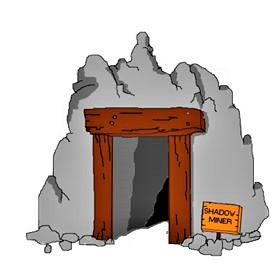
\includegraphics[%
			keepaspectratio]{../images/icone.jpg}%
			\vfill
		}
	}
}

\fboxrule=2pt
\newcommand\cincludegraphics[2][]{%
  \setbox0=\hbox{\includegraphics[#1]{#2}}%
  \abovebaseline[-.5\ht0]{\includegraphics[#1]{#2}}}

  
\renewcommand{\baselinestretch}{1}
\renewcommand{\partname}{}


\title{\textbf{{\Huge Manuel d'utilisation}}}
\author{
	\\
	\bsc{{\LARGE \bf ShadowMiner}} \\ \\ \\
	\bsc{{\LARGE \bf par ACCEr}} \\ \\
}
\date{{\LARGE \today}}

\pagestyle{fancy}
%\fancyfoot[L]{
\includegraphics{../images/ShadowMiners_logo_mini.png}} %50x33
\fancyfoot[L]{\cincludegraphics[scale=0.1]{../images/ShadowMiners_logo.png}} %50x33
\fancyfoot[R]{STRASBOURG 2022}
\fancyhead[R]{ACCEr}
\fancyhead[L]{Manuel d'utilisation}

\setcounter{tocdepth}{3}

\begin{document}
\AddToShipoutPicture*{\BackgroundPic}

\maketitle
\tableofcontents
%\listoftables
%\listoffigures

%################### INTRO

\fancypagestyle{plain}{}
\stepcounter{chapter}
\part{Introduction} 
\paragraph{} \hspace{0pt}


%################### INTRO


\newpage

%################### Qui sommes nous ?

\fancypagestyle{plain}{}
\stepcounter{chapter}
\part{Qui sommes nous ?}
\section{Présentation des membres du groupe}

\paragraph{~~~~Cédric (Chef de projet)} \hspace{0pt} \\
Je m’appelle Cédric FARINAZZO. Je suis originaire de la région parisienne. 
J’ai intégré EPITA Strasbourg sur un coup de chance. Depuis, je me passionne pour l’informatique. 
J’adore découvrir de nouveaux langages ou me lancer des défis. \\
Réaliser un jeu vidéo est un rêve pour tous le monde. Ce projet est donc une occasion en or de le réaliser. 
Dès décembre, j’ai donc proposé à Clément et Antoine de faire ce projet ensemble puis nous avons accueillis Edgar. \\
En tant que chef de projet, je donne donc le meilleur de moi-même afin de permettre la réussite de ce projet. \\


\paragraph{~~~~Antoine} \hspace{0pt} \\
Bonjour ! Je m'appelle Antoine mais ça tout le monde le sait à ce niveau du rapport.  
J'ai commencé à apprécier les jeux vidéo lorsque mon père m'a fait découvrir la série de 
jeux « Half-Life ». Depuis j'ai exploré nombres mondes imaginaires et j'ai continué à 
entretenir ma relation avec les jeux. \\
Mon premier jeu vidéo réalisé fut un Snake codé 
en Python dans le cadre de l'ISN au lycée. Ce fut plutôt une réussite donc je partais 
confiant sur un projet plus ambitieux tel que le ShadowMiner. J'ai bien fait de rejoindre le groupe. \\


\paragraph{~~~~Clément} \hspace{0pt} \\


\paragraph{~~~~Edgar} \hspace{0pt} \\



\section{L'origine du nom du groupe : \textit{ACCEr}}
\paragraph{} \hspace{0pt}
Le nom du groupe provient d’Antoine. A l’origine, nous nous appelions ACCer avant l’arrivée d’Edgar. 
« ACC » pour les initiales de nos prénoms et « er » pour porter confusion entre notre groupe 
et la société taïwanais ACER, constructeur informatique. \\ \\
A l’arrivée d’Edgar, on a décidé de mettre en majuscule le « e » de notre nom. \\
C’est ainsi qu’ACCEr est né.

\newpage

\section{Planning}
\paragraph{} \hspace{0pt}
Voici un rappel de notre planning annoncé dans le cahier des charges :
\\ \\
{\small
	\begin{tabular}{|p{7.2cm}|p{1.2cm}|p{1.2cm}|p{1.2cm}|}
		\hline
		Pourcentages des tâches & \multicolumn{3}{|c|}{jusqu'à la soutenance} \\ 
		\cline{2-4}
			& \no 1 & \no 2 & \no 3 \\
		\hline
		Création des préfabs de map pour les niveaux (murs, sol, porte, ..) & 75\% & 100\% & 100\% \\
		\hline
		Modélisation 3D pour de meilleurs graphismes (si possible) & 0\% & 75\% & 100\% \\
		\hline
		Script c\# animation & 30\% & 60\% & 100\% \\
		\hline
		Création des préfabs des joueurs & 100\% & 100\% & 100\% \\
		\hline
		Script c\# joueur & 50\% & 75\% & 100\% \\
		\hline
		Création de multiples niveaux (entre 20 et 40) & 10-20\% & 50\% & 100\% \\
		\hline
		Création du Shadow Miner et Script c\# pour l'IA du Shadow Miner & 30\% & 60\% & 100\% \\
		\hline
		Cinématique du jeu & 0\% & 50\% & 100\% \\
		\hline
		Son du jeu & 0\% & 30\% & 100\% \\
		\hline
		Menu du jeu & 0\% & 40\% & 100\% \\
		\hline
		Création du site internet et Hébergement en ligne & 40\% & 80\% & 100\% \\
		\hline
		Création du serveur multijoueurs & 40\% & 90\% & 100\% \\
		\hline
		Création des joueurs pour multijoueurs & 30\% & 90\% & 100\% \\
		\hline
		Création du système de map aléatoire pour le multijoueurs & 0\% & 20\% & 100\% \\
		\hline
		Compilation du jeu et enregistrement sur CD & 0\% & 0\% & 100\% \\
		\hline 
		\end{tabular}
	\label{Planning}	
}


%################### Qui sommes nous ?


\newpage

%################### ShadowMiner

\fancypagestyle{plain}{}
\stepcounter{chapter}
\part{Le jeu : ShadowMiner}
\section{Le mode solo}

\subsection[Scénario]{~~~~Scénario}
\paragraph{} \hspace{0pt}
\begin{quotation}
	Un mineur descend tôt le matin dans les derniers sous-sols de la mine, là où l’oxygène se fait rare. 
	Un mineur fou (le Shadow Miner) coupe les câbles de l’ascenseur. 
	Le mineur veut alors rejoindre la surface. Le Shadow Miner va alors vouloir l’en empêcher. \\
\end{quotation}

\subsection[Gameplay]{~~~~Gameplay}
\paragraph{} \hspace{0pt} \\
L’utilisateur incarne alors le mineur. \\
Le joueur devra donc progresser dans une série de niveaux de plus en plus difficiles. \\
Des pièges tels que des piques ou des traps seront là pour le ralentir. \\
Le ShadowMiner lui-même sera là pour le traquer et le capturer dans les niveaux les plus difficiles. \\
Chaque niveau symbolise un étage de la mine. Le joueur devra donc rejoindre un checkpoint 
qui symbolise la fin d’un niveau pour passer à l’étage suivant et donc au niveau suivant. \\
Le dernier niveau est donc la sortie de la mine. \\ 

\subsection[Progression du joueur]{~~~~Progression du joueur}
\paragraph{} \hspace{0pt} \\
Le joueur devra réussir le niveau actuel pour accéder au niveau suivant. \\ \\
La progression du joueur est visible en jeu et sur le site internet \url{https://accer.ddns.net} si le joueur a liée son compte au jeu. \\

\newpage

\section{Le mode multijoueurs}

\subsection[Prérequis]{~~~~Prérequis}
\paragraph{} \hspace{0pt} \\
Le joueur devra créer un compte pour pouvoir accéder au mode multijoueurs. \\
Ce compte pourra être créer sur le site internet \url{https://accer.ddns.net} ou dans le jeu lui-même Ainsi le joueur pourra 
consulter et modifier ses données depuis le site internet \url{https://accer.ddns.net} ou depuis le jeu. Ce système lui permet 
de jouer sur n’importe quel exécutable du jeu en conservant ses données. 
Cela accroit fortement la portabilité du jeu. \\

\subsection[Gameplay]{~~~~Gameplay}
\paragraph{} \hspace{0pt} \\
Le joueur rejoint tous d’abord un lobby où il doit attendre que trois joueurs 
soient connectés avant que la partie ne commence.

\paragraph{} \hspace{0pt} \\
Un joueur incarnera le ShadowMiner et devra tuer les deux autres joueurs qui 
incarneront deux mineurs voulant rejoindre la surface. Un des mineurs pourra 
s’enlever la vie et devenir un esprit de la mine qui contrôle les cloisons de 
la mine (porte, mur, gouffre) pour aider l’autre mineur. \\

\paragraph{~~~~Comment gagner ?} \hspace{0pt}
{\begin{itemize}
	\item Le ShadowMiner doit tuer tous les mineurs pour remporter la partie,
	\item Les mineurs doivent survivre jusqu’à la fin du minuteur pour remporter la partie. \\
\end{itemize}}

\subsection[Score du joueur]{~~~~Score du joueur}
\paragraph{} \hspace{0pt} \\
Le joueur gagnera en score à chaque victoire en mode multijoueurs. \\
Son score sera visible en jeu mais aussi sur le site internet \url{https://accer.ddns.net}. \\
Un classement des meilleurs joueurs est d’ailleurs disponible sur le site internet \url{https://accer.ddns.net}. \\


\newpage

\section{Le site internet}
\subsection[Hébergement]{~~~~Hébergement}
\paragraph{} \hspace{0pt} \\
L'adresse du site internet est \url{https://accer.ddns.net}. \\
Il est hébergé à Strasbourg chez Cédric sur un Raspberry pi modèle 3B+. \\
L’accès au site est assuré par un élastique qui maintient le câble Ethernet relié au Raspberry pi. \\

\subsection[Compte]{~~~~Compte}
\paragraph{} \hspace{0pt} \\
Il permet de créer, gérer son compte comme modifier son pseudo, sa description, son image de profil ou encore son mot de passe. \\

\subsection[L’onglet Shadow Miner]{~~~~L’onglet Shadow Miner}
\paragraph{} \hspace{0pt} \\
Cet onglet permet d’accéder à plusieurs pages : \\
{\begin{itemize}
	\item Une brève description du projet (\url{https://accer.ddns.net/?p=project})
	\item Les sources utilisées (\url{https://accer.ddns.net/?p=source})
	\item La liste de tous les rapport (\url{https://accer.ddns.net/?p=report})
	\item Une page permettant de voir l’avancement du projet \\
		(\url{https://accer.ddns.net/?p=progress})
	\item Une page de téléchargement de l’installateur du jeu \\
		(\url{ https://accer.ddns.net/?p=download}) \\
\end{itemize}}

\subsection[Accès depuis le jeu]{~~~~Accès depuis le jeu}
\paragraph{} \hspace{0pt} \\
Afin de pouvoir gérer son compte depuis le jeu, un serveur et un client ont été créé en C\#. \\
Le serveur écoute sur le port TCP 4247 (l’adresse est donc accer.ddns.net:4247). Ainsi le client, 
intégré au jeu, permet de créer un compte ou alors de se connecter, de modifier son pseudo, 
son mot de passe, sa description, son nom et prénom. \\
Il permet aussi de synchroniser la progression du joueur en mode solo ou le score du joueur 
en mode multijoueurs (pour lequel il est obligatoire de créer un compte). \\

%################### ShadowMiner

\newpage

%################### Réalisation individuelle

\fancypagestyle{plain}{}
\stepcounter{chapter}
\part{Réalisation individuelle}
\section*{Contexte}
\paragraph{} \hspace{0pt}


\newpage
\section{Antoine}
\subsection{Introduction}
\paragraph{} \hspace{0pt} 
Mes tâches pour ce projet furent la création des préfabs (objets complexes qui
serviront de base) pour les niveaux (murs, sol, porte, ..) et la création de multiples
niveaux. Elles ont été établies lors de la rédaction du cahier des charges début février. \\

\subsection{Description du travail}

\paragraph{} \hspace{0pt} 
Pour débuter le projet j'ai commencé par construire des préfabs. Le tout premier
objet que j'ai utilisé est un cube 3D. En le dupliquant puis en assemblant ses
copies j'ai construit un mur en pierre. Ce fut le début de l'ère des préfabs. \\@(\# antoine\_mur.png \#)\@  \\
Je construisis dans la foulée une table en bois. Les textures (bois et pierre)
proviennent d'un package gratuit de l'« asset-store ». Nous nous sommes ensuite
mis d'accord avec le groupe au sujet de cette plateforme : nous utiliserons le
moins possible son contenu. \\

\paragraph{} \hspace{0pt} 
Par la suite j'ai créé une flamme en utilisant le système de particule d'Unity3D, les
anciens élèves de 1ère année à EPITA nous avaient conseillés d'en abuser car les
particules plaisent beaucoup aux professeurs. Mythe ou réalité ? Quoi qu'il en soit
nous avons trouvé les flammes réussies et je m'en suis donc servi pour
confectionner des torches et des lanternes. J'avais donc respecté l'accord vis à vis
du contenu prémâché de l' «asset-store » d 'Unity3D. \@(\# antoine\_mineurtorche.png \#)\@ \\


\paragraph{} \hspace{0pt} 
Je continuai à le respecter en installant Blender. Ce logiciel m'a servi à créer des
rochers en modelant une sphère grâce à l'outil de sculpture. Après avoir transféré
les rochers sur Unity, j'ai ajouté un compostant de gravité pour provoquer des
éboulements dans le jeu. Cette phase de création se situe peu avant la première
soutenance du 14 mars 2018. \\


\paragraph{} \hspace{0pt} 
J'ai réalisé ma première interface utilisateur à ce moment. Il s'agit du premier menu
du jeu, composé de trois boutons : 1. Niveau un ; 2. Niveau deux ; 3. Multijoueur.
J'utilisai l'option « Add on click » d'Unity pour charger les scènes des trois niveaux
lorsque le joueur cliquait sur un bouton. Comme il n'y avait encore que trois
boutons j'ai écrit un script (C\#) pour chaque bouton. Le niveau 1 fut construit par
Clément et la scène multijoueur par Cédric. Je m'étais occupé du niveau 2. Ce
niveau commence dans un couloir peu éclairé (avec les murs construits
précédemment et quelques torches). Au bout du couloir sur la gauche on trouve un
escalier condamné qui représente l'accès au niveau suivant. Le joueur doit donc
continuer à droite et après quelques pas il se trouvera devant un énorme cratère
qui constitue la zone de minage. \@(\# antoine\_cratere.png \#)\@   \\


\paragraph{} \hspace{0pt} 
Fin avril la création d'autres niveaux commença. Je construisis un niveau avec un
sol qui s'écroule lorsque le joueur passe dessus et un niveau avec un passage
enflammé. A partir de ce moment les flammes infligent des dégâts aux joueurs. Le
sol qui s'effondre et les flammes interagissent avec le mineur (personnage du
joueur) via leur « collider » (composant qui, en vulgarisant, permet de gérer les
colisions entre les objets). Ces niveaux atteignent leur objectif principal du point de vue de
l'originalité mais ils sont bien trop court pour constituer des niveaux à eux seuls,
c'est pourquoi j'ai créer un grand niveau modèle qui a été dupliqué 19 fois. Les
deux mini-niveaux mentionnés ci-dessus ont donc été intégrés à 2 des clones du
niveau modèle. \\


\paragraph{} \hspace{0pt}
Le niveau modèle est un niveau assez simple sur le plan du gameplay mais plus
grand et plus impressionnant (si si je vous assure). Il débute avec un couloir
comme les deux premiers niveaux construits avant la première soutenance début
mars. Le couloir passe devant une porte qui cache les toilettes, il continue jusqu'à
la salle de détente avec tables, étagères, tabourets et un jukebox. Le jukebox
permet d'activer/désactiver la musique ambiante. Après cette salle le couloir
reprend et se termine dans un espace de minage avec des cagettes de pépites
d'or et des murs pleins de minerais. \@(\# antoine\_pepite.png \#)\@   \\


\paragraph{} \hspace{0pt} 
Dans le même temps j'ai commencé la réalisation d'un niveau pour le mode
multijoueur. Le plan du niveau a été réalisé sur Paint (logiciel de dessin) et ce
niveau contient un labyrinthe, des faux murs (qui se comportent comme des
portes), des passages sous-terrains et un pont tournant. Le labyrinthe est généré
automatiquement lors du lancement du salon multijoueur. Chaque terrain possède
donc une partie connue et une autre inconnue. \\


\paragraph{} \hspace{0pt} 
Pour le menu du jeu j'ai d'abord assemblé boutons et textes pour créer une
interface de connexion au serveur, puis d'inscription. J'ai ensuite repris la première
scène du choix des niveaux (avec les trois boutons rappelez vous) et j'ai rajouté
les 17 autres niveaux (les clones du niveau modèle).\@(\# antoine\_choixniveau.png \#)\@ Cédric, étant responsable de
la création du site internet « accer.ddns.net», m'a aidé à rédiger le script qu'il avait créé permettant 
d'échanger des données avec le serveur et d'autres aspects du menu. Ainsi le script prends
en paramètre une liste des niveaux et des boutons et charge la scène adaptée
lorsqu'on clique sur un des boutons. Nous avons aussi créer la scène « mon
profil » qui permet à l'utilisateur d'accéder aux informations de son compte
(prénom, nom, adresse mail, mot de passe, description et pseudo) et de les
modifier. \@(\# antoine\_myaccount.png \#)\@ \\


\paragraph{} \hspace{0pt} 
Pour terminer, ma dernière contribution au projet (avant la soutenance finale car je
prévois d'améliorer le jeu par la suite) fut de créer d'autres mini-niveaux pour les
ajouter aux copies du terrain modèle et rendre chaque niveau différent. \\


\subsection{Apports personnels}
\paragraph{} \hspace{0pt}
Ce projet m'a apporté énormément de choses ! Pour commencer, réaliser un projet
de plusieurs mois impose un temps de travail conséquent. Ce temps de travail est
d'autant plus optimisé qu'il est régulier, nous en avons fait l'expérience. J'ai donc
appris à mieux me rendre compte de mes capacités, à optimiser les heures avec le
groupe, les heures en salle machine et les heures de rêverie à imaginer les
prochaines étapes du projet. \\

\paragraph{} \hspace{0pt}
Au fur et à mesure de l'avancement du projet j'ai rencontrée plusieurs difficultés.
Par exemple mes scripts C\# qui ne prenaient pas de variables dans Unity, les
flammes qui ne faisaient aucun dégâts au joueur ou encore les murs qui
tremblaient sur leur point d'intersection. Tous ces problèmes furent résolus grâce
au soutien des autres membres du groupe. Cependant il est arrivé que certains
soucis ne trouvent pas de solutions, mais nous avons toujours pu contourner ces
complications. \\


\paragraph{} \hspace{0pt} 
De plus comme nous apprenions chacun à notre façon, à l’unisson nous
possédions plusieurs méthodes pour une seule tâche et chacun pouvait apprendre
des autres. Dans la partie précédente (Description du travail) j'ai témoigné avoir
utilisé l'utilitaire « add on click » d'Unity alors que par la suite Cédric m'a montré
que la fonction « Button.OnClick.addListener() » faisait la même chose. Cela évitait de devoir
ajouter les vingts boutons de niveaux pour le choix du terrain en mode solo. \\


\paragraph{} \hspace{0pt} 
Ce jeu-vidéo permet aussi de laisser une trace de nos efforts et de notre travail
d'équipe . Nous pourrons continuer à travailler dessus pendant notre temps libre
(si on a un tant soit peu de temps libre) et tout comme certains projets d'anciennes
promotions d'EPITA sont restés disponible sur Internet, le notre rejoindra cette
grande famille. Ce sera une pierre en plus dans l'édifice. \\


\subsection{Conclusion}
\paragraph{} \hspace{0pt}
Mes tâches ont donc été réalisées. Le menu du jeu est opérationnel, les niveaux
sont au nombre de vingts (et un pour le multijoueur). \\


\newpage
\section{Cédric}
\paragraph{} \hspace{0pt}


\newpage
\section{Clément}
\paragraph{} \hspace{0pt}


\newpage
\section{Edgar}
\paragraph{} \hspace{0pt}
Nous sommes en septembre, le projet est annoncé à toute la classe. 
J’étais déjà particulièrement enthousiaste avant, je connaissais l’existence du projet. 
En septembre, ma motivation pour le projet était plutôt haute, je commençais à avoir quelques idées 
qui me paraissaient sympathique, bonne, d’autres vraiment mauvaise. Dans mon coin, 
j’avais noté quelques idées possibles que je trouvais bonnes comme un logiciel avec plein de jeux de société, 
un jeu dans un endroit plutôt lugubre avec un monstre, un jeu de combat et quelques autres. 
Mon souhait était clairement de créer un jeu de toutes pièces avec mes camarades, 
je voulais voir et savoir comment créer quelque chose qui me paraissait complexe. 
L’aspect " construction"  était surement la chose la plus intéressante à ce moment où notre aventure 
n’avait pas encore commencé. En Octobre-Novembre, je commence à me chercher un groupe avec lequel je pourrais 
m’entendre et travailler, je cherchais un groupe qui pouvait avoir les qualités d’un bon groupe 
qui sont selon moi, l’entente, la communication, la notion de travail, l’organisation. 
La recherche de ce groupe fut complexe et vers décembre, un groupe se propose de m’accueillir, 
le groupe ACCEr était créé. Notre groupe était alors composé de Cédric Farinazzo, Antoine Claudel, 
Clément Languerre et de ma personne. Je ne rappelle pas parfaitement si nous nous connaissions 
bien avant de venir en groupe, je connaissais un peu Cédric et Clément pour avoir fait 
la pré-rentrée avec eux, je n’ai aucun souvenir de bien connaître Antoine avant le projet. 
Aujourd’hui je pense que nous nous connaissons plutôt bien. \\


\paragraph{} \hspace{0pt}
Le nom du groupe est venu d'Antoine, si je me souviens bien il avait mis les initiales de nos 
prénoms respectifs dans l’ordre alphabétique (ACCE), il rajouta alors un r minuscule pour 
que cela ressemble au constructeur informatique mondialement connu Acer. Nous n’avions pas 
d’autre idée alors celle-ci fut retenue. Nous avons créé une conversation en groupe pour 
mieux communiquer, nous commençâmes à penser à notre idée de jeu chacun de notre côté et 
se dire nos idées principales pour le projet. Nous sommes en janvier, le projet démarre, 
Cédric propose une idée de jeu style Battle Royale, ce qui est particulièrement à la mode 
à ce moment de l’année, Clément propose un jeu dans une mine avec un monstre qui était une 
partie de mes idées, je trouvais cette idée excellente, selon moi c’était la meilleure idée, 
l’idée de Shadow Miner était née. \\


\paragraph{} \hspace{0pt}
Notre aventure commence, le cahier des charges se fait dans les temps avec nos idées, nous faisons une 
ou deux réunions de projet, où chacun de nous donne ses idées. Certaines idées vont un peu dans l'utopie 
pour un projet comme celui ci mais ces idées utopiques montrent quelque chose d'une importance cruciale 
voire vitale, nous étions motivés et enthousiastes. Un florilège d'idée sort de nos réunions, nous avons 
alors choisi les meilleurs selon nous et elles apparaissent aujourd'hui dans notre cahier des charges, 
même si certaines choses ont été modifiées depuis.  \\


\paragraph{} \hspace{0pt}
Entre le début de la première soutenance, nous avons commencé le projet, pour moi un peu difficilement, 
j'ai pas réussi à utilisé Unity à cause de mon ordinateur un peu vieux. \\
À présent je vais vous expliquer mon travail 
personnel sur le projet, où est-ce que j’ai œuvré à travers ce projet tout au long de l’année. \\


\paragraph{} \hspace{0pt}
Avant la première soutenance, je me suis énormément concentré pour la modélisation 3D ainsi que le personnage 
du mineur et du Shadow Miner, j’ai appris comment modéliser un personnage en 3D sur le logiciel Blender, 
cela m’a pris plusieurs heures pour avoir quelque chose que je trouvais pas si mal où je pouvais mettre 
des animations même si c’était un personnage et sans visage sans mains et sans pieds. J’avais créé un squelette 
en 3D qui pouvez recueillir des animations , ensuite je lui aie fait des muscles à ce personnage mais pour 
avoir un homme vraiment réaliste qui ressemble à quelque chose, je devais sûrement prendre un temps de travail 
considérable peut-être 10 fois plus que ce que j’avais mis dans la création de ce personnage en 3D. 
J’ai appris comment modélisé en 3D et cela m’intéressé donc j’étais content et heureux de l’avoir fait. 
Néanmoins le travail fourni ne correspondait pas aux attentes de mes camarades en effet il était particulièrement 
laid. \\
C’était sûrement trop dur de créer un monstre 
ou un mineur donc nous sommes partis chercher des personnages de mineur et de monstres sur Internet dans des 
banques de données. Un camarade m’avez parlé du site Mixamo, je crois avoir passé quelques heures sur ce site 
pour l’analyser pour trouver des choses qui était bien pour le début notre projet et avec Cédric nous avons 
trouvé le personnage et le physique de notre monstre (qui a été remplacé par la suite) et pour la soutenance nous 
avons montré que nous pouvions déjà l’animer malheureusement il était sans couleur, il était tout blanc. 
Quelques jours avant la première soutenance j’ai commencé utiliser Unity sur un des ordinateurs du campus. 
Bien évidemment mes connaissances et mes compétences sur ce logiciel était totalement en retard par rapport à mes 
camarades même si j’ai essayé de rattraper tant bien que mal ce retard. J’ai essayé de modéliser certaines 
choses sur Blender tels que des roches des amas de roches, en fait tout était déjà fait mais aujourd’hui, 
j’ai appris à le faire et c’est cela le plus important. \\
La première soutenance approchait à grands pas, 
la veille (et toute la nuit) Cédric et Clement ont fait un travail exceptionnel que je me permet de souligner car ils ont œuvraient 
comme des chefs pour obtenir un très bon résultat. \\

\paragraph{} \hspace{0pt}
Pendant la période entre la première et la deuxième soutenance, 
nous avons fait du bon travail. Personnellement je me suis focalisé sur 
le son du jeu parce que c’est quelque chose qui m’intéresse énormément, je voulais absolument enregistrer 
des sons ou aller en prendre sur des banques de données en ligne, pouvoir les modifier pouvoir avoir une 
musique de fond qui était bien pour le jeu. Tout l’aspect sonore et audio du projet était sûrement 
la chose qui m’intéressait le plus. Pendant quelques jours j’ai cherché des sons qui était idéaux pour le jeu, 
comme le bruit d’un éboulement de cailloux dans la mine, le cri du monstre les bruits de pas, les bruits de pas 
quand le mineur court. \\
J’ai vrai une dernière chose sur leçon 
qui était les musiques de fond. Lors de la première soutenance pour montrer que nous pouvions mettre de la 
musique nous avions mis une musique qui rendait bien mais qui était particulièrement énervante au bout de 30 secondes 
d’écoute. Il nous fallait absolument une voire deux autres musiques de fond. C’est un ami du nom de 
Nicolas Maschiocchi, que nous remercions particulièrement, qui a composé une musique, c’était une musique 
qui collait parfaitement mange avec certains temps plutôt calme avec du piano, et d’autres temps très puissant 
avec des cuivres et des violons qui peuvent très bien rendre le jeu plus vivant. J’ai découpé la musique en 
quelques parties évidemment, je garde l’original précieusement. L’aspect musical et sonore du jeu m’a fait 
comprendre à quel point le son est important dans un jeu l’immersion est beaucoup plus présente, grâce à 
cette musique le jeu en devient plus puissant et c’est une excellente chose pour nous. \\
Cette Fois-ci nous avons vraiment bien travaillé bien communiquer nous avions un travail qui était bon à mes yeux 
le rapport et le plan de soutenance a été fait dans les temps, nous n’avions pas de retard. J’ai fait aussi avec 
Antoine le PowerPoint de la présentation puis nous l’avons tous un peu modifié et cette fois-ci nous étions vraiment 
prêt et préparer pour la deuxième soutenance et elle s’est très bien passé. Nous avons pu montrer le fruit de notre 
travail notre projet n’était pas encore terminé mais vu le travail déjà accompli nous étions plutôt fier. \\


\paragraph{} \hspace{0pt}
Et aujourd’hui nous écrivons notre rapport de projet cela nous rappelle et remémore des souvenirs de travail et 
de groupe certains moments furent stressant comme la préparation avant les soutenances
, d’autres agréable comme des moments de rigolade dans le groupe où nous blaguions entre nous. Le groupe 
ACCEr a fait son projet avec envie à mes yeux, en tout cas c’est mon cas je suis resté motivé pour ce projet, 
j’ai appris plein de choses très intéressantes pas forcément sur le plan informatique mais aussi sur le plan 
personnel j’ai appris à communiquer dans un groupe que je ne connaissais que très peu aujourd’hui j’aime 
travailler avec ses trois messieurs qui m’entourent. Nous espérons avoir fait un travail qui peut convenir 
au jury et nous espérons aussi à répondre à leurs attentes. \\


\newpage
\section{Conclusion}
\paragraph{} \hspace{0pt}


%################### Réalisation individuelle

\newpage

%################### Sources et remerciements

\fancypagestyle{plain}{}
\stepcounter{chapter}
\part{Sources et remerciements}

\section{Sources}
\paragraph{} \hspace{0pt}
N'etant pas des experts en modélisation 3D , nous avons dû trouver nos personnages sur internet : 
{\begin{itemize}
	\item Le mineur provient des standarts assets de Unity 4.x, nous avons juste récupéré le modele 3D et les animations, 
	car nous n'avons pas le droit de récupérer de script. De plus, les scripts de l'assets étaient en Javascript(Unityscript).
	\item les textures sur les objets et les sols et le modèle 3D du ShadowMiner proviennent de l'Assets Store. \\
\end{itemize}} 

Voici aussi les sources des musique et des effets sonores du jeu : \\
{\begin{itemize}
	\item \url{http://www.universal-soundbank.com/bruitdepas.htm}
	\item \url{http://www.universal-soundbank.com/terre.htm}
	\item \url{http://www.universal-soundbank.com/cris.htm} \\
\end{itemize}} 

\section{Technologies utilisées}
\paragraph{} \hspace{0pt}
Pour réaliser ce projet, nous avons dû coder dans plusieurs langages : 
{\begin{itemize}
	\item C\# pour le jeu, 
	\item HTML, CSS, JavaScript, PHP, MYSQL pour le site internet,
	\item \LaTeX ~ pour les rapports. \\
\end{itemize}}

\paragraph{} \hspace{0pt}
Nous avons aussi utilisé quelques Framework  afin de réaliser rapidement le design du site internet :
{\begin{itemize}
	\item Le framework JQuery (\url{https://jquery.com/}). pour simplifier la mise en place du javascript,
	\item Materialize css (\url{https://materializecss.com/}) permettant de donner un style au site simplement. \\
\end{itemize}}

\section{Remerciements}
\paragraph{} \hspace{0pt}
Nous remercions aussi Nicolas Masciocchi de nous avoir gentimment autorisé à utiliser sa musique comme musique de fond. \\

%################### Sources et remerciements

\newpage

%################### Quelques images du jeu

\fancypagestyle{plain}{}
\stepcounter{chapter}
\part{Quelques images du jeu}


%################### Quelques images du jeu

\newpage

%################### Conclusion

\fancypagestyle{plain}{}
\stepcounter{chapter}
\part{Conclusion}
\paragraph{} \hspace{0pt}
Conclusion

%################### Conclusion

\newpage

%################### Glossaire

\fancypagestyle{plain}{}
\stepcounter{chapter}
\part{Glossaire}
\paragraph{} \hspace{0pt}


%################### Glossaire

\end{document}